\section{Rendimiento del sistema}
\label{sec:rendimiento_sistema}

Para cada número de cámaras se ejecutó una sesión de cinco minutos en los dos
escenarios. Los valores de CPU y RAM son la mediana de las muestras que la
telemetría recoge cada 5\,s; el análisis estadístico se realizó con
NumPy~\cite{numpy_2020} y SciPy~\cite{scipy_2020}. El consumo energético se midió
con el sensor \ac{RAPL}~\cite{khan2018rapl} del procesador, que devuelve el consumo
real del paquete CPU en vatios. Los valores de las gráficas descuentan el consumo
en reposo de cada entorno para mostrar únicamente el coste atribuible a Voctomix.

\begin{figure}[H]
  \centering
  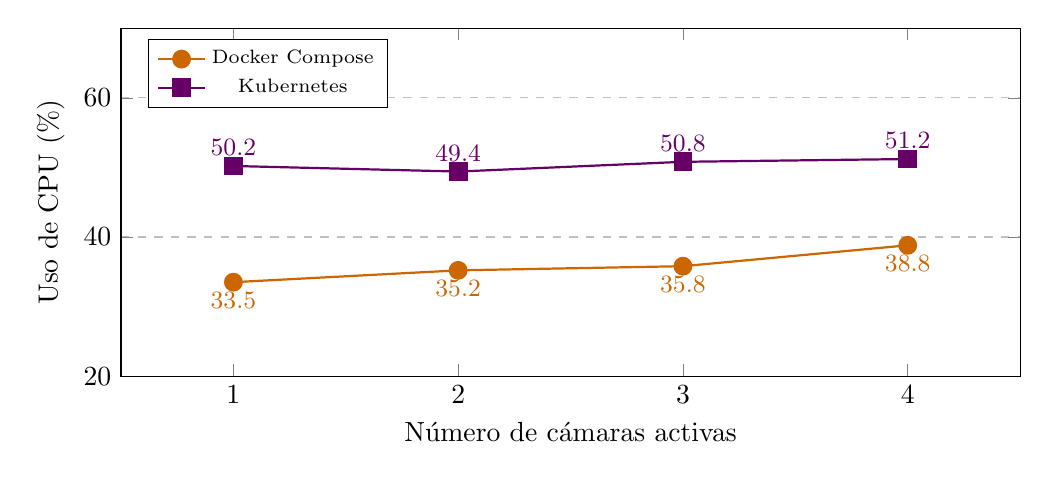
\begin{tikzpicture}
    \begin{axis}[
      width=13cm, height=6cm,
      xlabel={Número de cámaras activas},
      ylabel={Uso de CPU (\%)},
      xtick={1,2,3,4},
      xmin=0.5, xmax=4.5,
      ymin=20, ymax=70,
      ymajorgrids=true, grid style=dashed,
      mark size=3pt,
      legend style={at={(0.03,0.97)}, anchor=north west, font=\scriptsize},
    ]
      \addplot[color=orange!80!black, mark=*, thick,
               nodes near coords,
               every node near coord/.style={font=\small, anchor=north}]
        coordinates {(1,33.5) (2,35.2) (3,35.8) (4,38.8)};
      \addplot[color=violet!80!black, mark=square*, thick,
               nodes near coords,
               every node near coord/.style={font=\small, anchor=south}]
        coordinates {(1,50.2) (2,49.4) (3,50.8) (4,51.2)};
      \legend{Docker Compose, Kubernetes}
    \end{axis}
  \end{tikzpicture}
  \caption{Uso de CPU en función del número de cámaras activas.}
  \label{fig:cpu_camaras}
\end{figure}

En Docker, la CPU sube de 33{,}5\,\% con una cámara a 38{,}8\,\% con cuatro, un
incremento de 5{,}3 puntos que refleja directamente el coste de añadir cada
fuente en GStreamer. En Kubernetes, la CPU se mantiene prácticamente plana en
torno al 50\,\% sin importar el número de cámaras. Esto se debe a que Minikube
ejecuta en el mismo equipo los cuatro procesos del plano de control del clúster:
\texttt{kube-apiserver}, \texttt{etcd}, \texttt{kube-scheduler} y
\texttt{kube-controller-manager}. Estos procesos elevan el consumo del sistema
hasta el 50{,}2\,\% incluso con una sola cámara activa, frente al 33{,}5\,\% que
registra Docker en las mismas condiciones. El trabajo real de mezcla de vídeo es
el mismo en los dos entornos, pero en Kubernetes queda enmascarado por este
consumo fijo de los procesos de orquestación.

\begin{figure}[H]
  \centering
  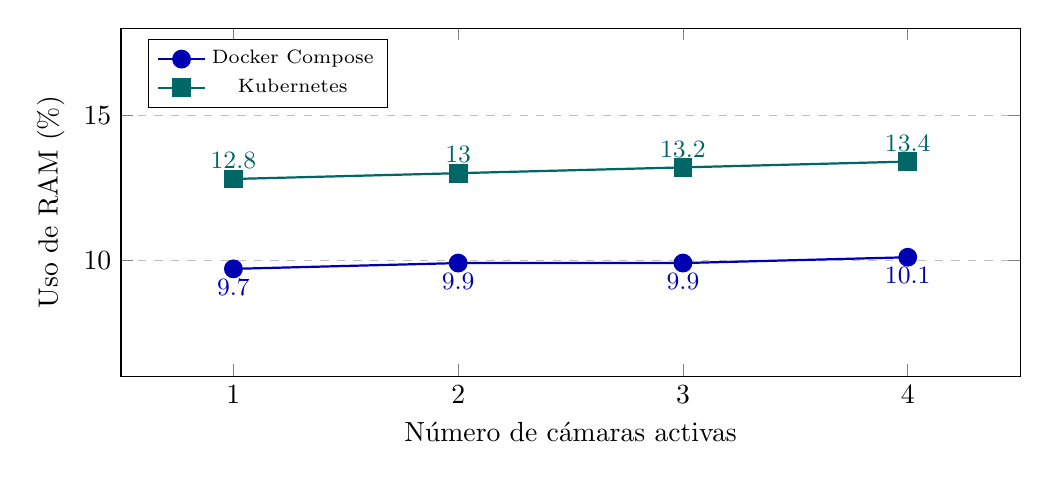
\begin{tikzpicture}
    \begin{axis}[
      width=13cm, height=6cm,
      xlabel={Número de cámaras activas},
      ylabel={Uso de RAM (\%)},
      xtick={1,2,3,4},
      xmin=0.5, xmax=4.5,
      ymin=6, ymax=18,
      ymajorgrids=true, grid style=dashed,
      mark size=3pt,
      legend style={at={(0.03,0.97)}, anchor=north west, font=\scriptsize},
    ]
      \addplot[color=blue!70!black, mark=*, thick,
               nodes near coords,
               every node near coord/.style={font=\small, anchor=north}]
        coordinates {(1,9.7) (2,9.9) (3,9.9) (4,10.1)};
      \addplot[color=teal!80!black, mark=square*, thick,
               nodes near coords,
               every node near coord/.style={font=\small, anchor=south}]
        coordinates {(1,12.8) (2,13.0) (3,13.2) (4,13.4)};
      \legend{Docker Compose, Kubernetes}
    \end{axis}
  \end{tikzpicture}
  \caption{Uso de RAM en función del número de cámaras activas.}
  \label{fig:ram_camaras}
\end{figure}

El uso de memoria apenas varía al añadir cámaras: Docker pasa de 9{,}7\,\% a
10{,}1\,\% y Kubernetes de 12{,}8\,\% a 13{,}4\,\%. La diferencia de unos
3 puntos entre entornos corresponde a la memoria que ocupa el plano de control
de Kubernetes. En ambos casos el consumo es prácticamente plano, lo que indica
que GStreamer reutiliza los búferes internos y que añadir cámaras no incrementa
el uso de memoria de forma significativa.

\begin{figure}[H]
  \centering
  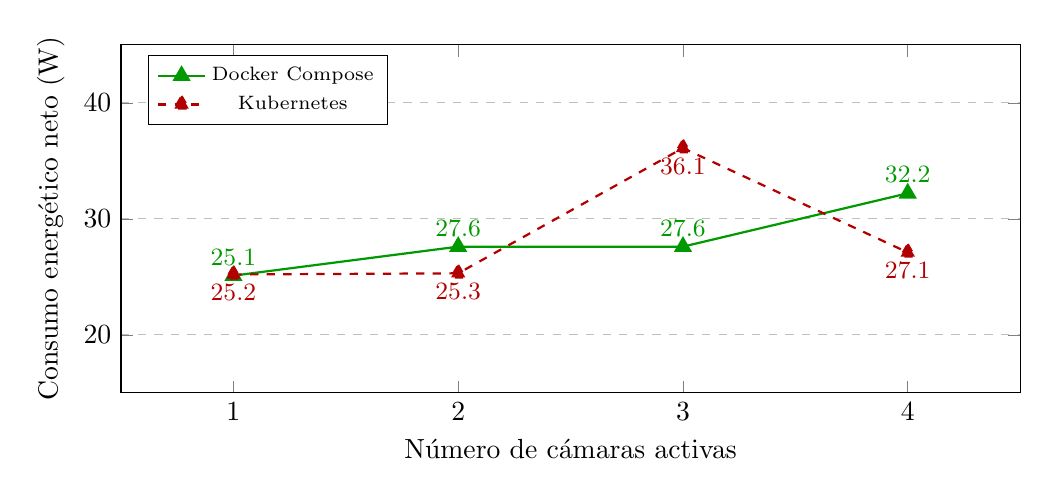
\begin{tikzpicture}
    \begin{axis}[
      width=13cm, height=6cm,
      xlabel={Número de cámaras activas},
      ylabel={Consumo energético neto (W)},
      xtick={1,2,3,4},
      xmin=0.5, xmax=4.5,
      ymin=15, ymax=45,
      ymajorgrids=true, grid style=dashed,
      mark size=3pt,
      legend style={at={(0.03,0.97)}, anchor=north west, font=\scriptsize},
    ]
      \addplot[color=green!60!black, mark=triangle*, thick,
               nodes near coords,
               every node near coord/.style={font=\small, anchor=south}]
        coordinates {(1,25.1) (2,27.6) (3,27.6) (4,32.2)};
      \addplot[color=red!70!black, mark=triangle*, thick, dashed,
               nodes near coords,
               every node near coord/.style={font=\small, anchor=north}]
        coordinates {(1,25.2) (2,25.3) (3,36.1) (4,27.1)};
      \legend{Docker Compose, Kubernetes}
    \end{axis}
  \end{tikzpicture}
  \caption{Consumo energético neto medido por RAPL en función del número de
           cámaras activas (descontado el baseline de cada entorno).}
  \label{fig:energia_camaras}
\end{figure}

El consumo neto atribuible a Voctomix es similar en los dos entornos: entre 25 y
32\,W en Docker y entre 25 y 36\,W en Kubernetes. El rango más amplio en
Kubernetes se debe a que el baseline del plano de control de Minikube no es
constante, sino que varía entre 59 y 63\,W según la actividad interna del
clúster, lo que introduce dispersión en los valores netos. En términos de consumo
total, Docker alcanza unos 50\,W con cuatro cámaras, el 30\,\% del \ac{TDP} del
procesador (165\,W), con margen suficiente para no saturarlo. Kubernetes supera
los 90\,W al sumar el trabajo de Voctomix y el del plano de control.

Este coste extra de Kubernetes es específico del uso de Minikube como clúster
local. En un despliegue sobre un clúster gestionado en la nube (Amazon \ac{EKS},
Google \ac{GKE} o Azure \ac{AKS}) el plano de control corre en servidores del
proveedor y los recursos disponibles para Voctomix serían equivalentes a los del
escenario Docker Compose.

En cuanto al ancho de banda, cada fuente RAW~I420 a 1080p25 genera 622\,Mbps.
Con cuatro cámaras activas, el tráfico total es de 2{,}49\,Gbps, que circula
íntegramente por la red interna del equipo, sin atravesar ninguna tarjeta de red
física, tanto en Docker como en Kubernetes.

\section{Latencia del sistema}
\label{sec:latencia_sistema}

Este apartado analiza los tiempos de respuesta del sistema: el tiempo necesario
para el arranque completo y la latencia de las operaciones de control que el
operador realiza durante la retransmisión. La tabla~\ref{tab:latencia_arranque}
resume los valores obtenidos con cuatro fuentes activas en cada escenario.

\begin{table}[H]
  \centering
  \caption{Tiempos de respuesta con cuatro cámaras activas.}
  \label{tab:latencia_arranque}
  \small
  \begin{tabular}{|l|c|c|}
    \hline
    \textbf{Métrica} & \textbf{Docker Compose} & \textbf{Kubernetes} \\
    \hline
    Tiempo arranque sistema (s)       & $\approx$20 & $\approx$90 \\
    \hline
    Tiempo pods/servicios listos (s)  & $\approx$15 & $\approx$60 \\
    \hline
    Latencia conmutación mediana (ms) & 1{,}5       & 1{,}8 \\
    \hline
    Latencia conmutación p95 (ms)     & 2{,}3       & 2{,}6 \\
    \hline
  \end{tabular}
\end{table}

El tiempo de arranque muestra una diferencia clara entre entornos. Docker Compose
levanta todos los servicios en unos 20\,s y, tras 15\,s adicionales para que
voctocore supere el \textit{healthcheck}, el sistema ya está listo para procesar
señal. Kubernetes necesita unos 90\,s para arrancar el clúster Minikube y otros
60\,s hasta que todos los pods están en estado \textit{Ready}, lo que suma algo
más de 2 minutos con imágenes ya descargadas. Este arranque más largo es asumible
en producción, ya que el sistema se despliega una sola vez antes del evento y
permanece activo durante toda la retransmisión.

\subsection{Latencia de conmutación}
\label{sec:latencia_conmutacion}

Se automatizaron 30 cambios de fuente consecutivos en cada entorno y se midió
el tiempo entre el envío del comando \texttt{set\_video\_a} y la respuesta
\texttt{video\_status} de voctocore, que se emite cuando GStreamer ha completado
el cambio. Como el vídeo es RAW~I420 sin compresión, no hay ningún búfer de
códec que añada retardo.

\begin{figure}[H]
  \centering
  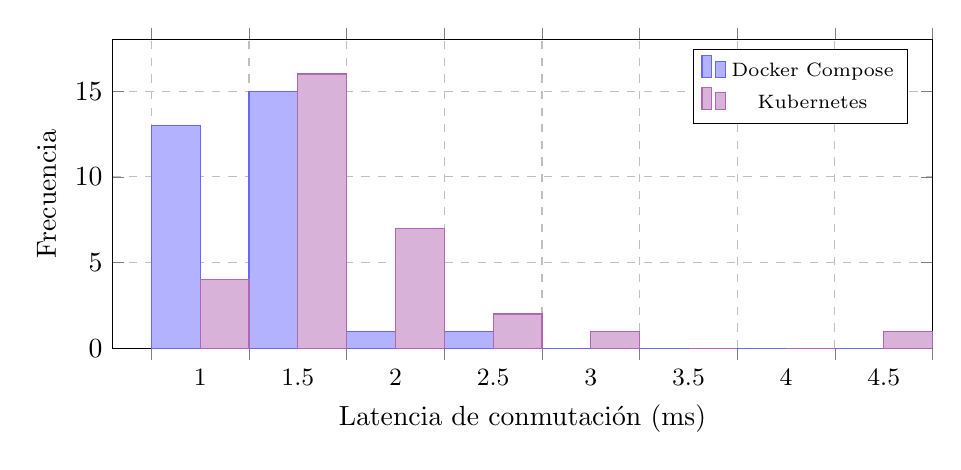
\begin{tikzpicture}
    \begin{axis}[
      ybar interval,
      width=12cm, height=5.5cm,
      xlabel={Latencia de conmutación (ms)},
      ylabel={Frecuencia},
      xtick={1.0,1.5,2.0,2.5,3.0,3.5,4.0,4.5,5.0},
      xticklabel style={font=\small},
      xmin=0.8, xmax=5.0,
      ymin=0, ymax=18,
      ymajorgrids=true, grid style=dashed,
      bar width=0.5,
      legend style={at={(0.97,0.97)}, anchor=north east, font=\scriptsize},
    ]
      \addplot[fill=blue!30, draw=blue!60]
        coordinates {(1.0,13) (1.5,15) (2.0,1) (2.5,1) (3.0,0) (3.5,0) (4.0,0) (4.5,0) (5.0,0)};
      \addplot[fill=violet!30, draw=violet!60]
        coordinates {(1.0,4) (1.5,16) (2.0,7) (2.5,2) (3.0,1) (3.5,0) (4.0,0) (4.5,1) (5.0,0)};
      \legend{Docker Compose, Kubernetes}
    \end{axis}
  \end{tikzpicture}
  \caption{Distribución de latencias de conmutación ($n=30$ mediciones por entorno).}
  \label{fig:latencia}
\end{figure}

\begin{table}[H]
  \centering
  \caption{Estadísticos de latencia de conmutación.}
  \label{tab:latencia_stats}
  \small
  \begin{tabular}{|l|c|c|}
    \hline
    \textbf{Estadístico} & \textbf{Docker} & \textbf{Kubernetes} \\
    \hline
    Mínimo   & 1{,}0\,ms & 1{,}4\,ms \\
    \hline
    Mediana  & 1{,}5\,ms & 1{,}8\,ms \\
    \hline
    Máximo   & 2{,}7\,ms & 4{,}7\,ms \\
    \hline
    $<$ 45\,ms (\ac{ITU-R} BT.1359-1) & 30\,/\,30 & 30\,/\,30 \\
    \hline
  \end{tabular}
\end{table}

El 100\,\% de las conmutaciones se resuelve en menos de 5\,ms en los dos
entornos. Un fotograma a 25\,fps dura 40\,ms, así que cualquier cambio por
debajo de ese valor es imperceptible para el espectador. La
Recomendación~\ac{ITU-R} BT.1359-1~\cite{itur_bt1359_1998} establece 45\,ms
como el umbral a partir del cual el ojo humano detecta desincronización entre
audio y vídeo: la mediana de Docker (1{,}5\,ms) queda 27~veces por debajo de
ese límite, y la de Kubernetes (1{,}8\,ms), 25~veces. La ligera diferencia
entre entornos se debe al salto adicional del \textit{port-forward} de kubectl
y no tiene impacto en producción.

\subsection{Latencia de transición de composite}
\label{sec:latencia_transicion}

Cambiar de modo de composición (de pantalla completa a \ac{PIP}, por ejemplo)
es diferente a cambiar de cámara: GStreamer tiene que animar la mezcla entre
dos modos fotograma a fotograma, y para hacerlo de forma sincronizada espera
al siguiente ciclo de procesado del pipeline, que ocurre cada 40\,ms a 25\,fps.
Se realizaron 32 mediciones en cada entorno ciclando entre los cuatro modos
disponibles. La figura~\ref{fig:latencia_transicion} muestra las distribuciones
y la tabla~\ref{tab:comparativa_latencias} compara los dos tipos de operación.

\begin{figure}[H]
  \centering
  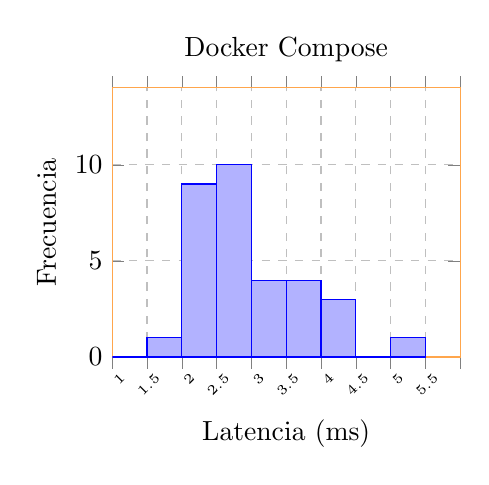
\begin{tikzpicture}
    \begin{axis}[
      ybar interval,
      width=6cm, height=5cm,
      title={Docker Compose},
      xlabel={Latencia (ms)},
      ylabel={Frecuencia},
      xtick={1.0,1.5,2.0,2.5,3.0,3.5,4.0,4.5,5.0,5.5,6.0},
      xticklabel style={font=\tiny, rotate=45, anchor=east},
      xmin=1.0, xmax=6.0,
      ymin=0, ymax=14,
      ymajorgrids=true, grid style=dashed,
      bar width=0.5,
      fill=orange!40, draw=orange!70,
    ]
      \addplot coordinates {(1.0,0)(1.5,1)(2.0,9)(2.5,10)(3.0,4)(3.5,4)(4.0,3)(4.5,0)(5.0,1)(5.5,0)};
    \end{axis}
  \end{tikzpicture}
  \hspace{1cm}
  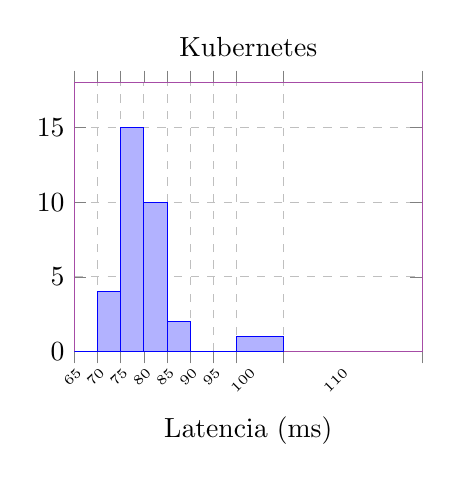
\begin{tikzpicture}
    \begin{axis}[
      ybar interval,
      width=6cm, height=5cm,
      title={Kubernetes},
      xlabel={Latencia (ms)},
      xtick={65,70,75,80,85,90,95,100,110,140},
      xticklabel style={font=\tiny, rotate=45, anchor=east},
      xmin=65, xmax=140,
      ymin=0, ymax=18,
      ymajorgrids=true, grid style=dashed,
      bar width=5,
      fill=violet!40, draw=violet!70,
    ]
      \addplot coordinates {(65,0)(70,4)(75,15)(80,10)(85,2)(90,0)(95,0)(100,1)(110,0)};
    \end{axis}
  \end{tikzpicture}
  \caption{Distribución de latencias de transición de composite ($n=32$ por entorno).
           Nótese la diferencia de escala: Docker en el rango 1--6\,ms,
           Kubernetes en el rango 65--140\,ms.}
  \label{fig:latencia_transicion}
\end{figure}

\begin{table}[H]
  \centering
  \caption{Comparativa de latencia mediana: conmutación de fuente vs.\ transición de composite.}
  \label{tab:comparativa_latencias}
  \small
  \begin{tabular}{|l|c|c|}
    \hline
    \textbf{Operación} & \textbf{Docker Compose} & \textbf{Kubernetes} \\
    \hline
    Conmutación de fuente   & 1{,}5\,ms &  1{,}8\,ms \\
    \hline
    Transición de composite & 2{,}8\,ms & 79{,}8\,ms \\
    \hline
  \end{tabular}
\end{table}

En Docker, ambas operaciones son casi iguales de rápidas (1,5\,ms vs 2,8\,ms)
porque la CPU está libre y GStreamer alcanza el siguiente ciclo sin esperar.
En Kubernetes, la conmutación sigue siendo igual de rápida (1,8\,ms), pero la
transición sube a 79,8\,ms: con la CPU al 50\,\% ocupada por el plano de
control, el pipeline llega tarde al primer ciclo y tiene que esperar al
siguiente (2 ciclos $\times$ 40\,ms $=$ 80\,ms). Es perceptible para el
operador, pero la animación se ejecuta correctamente y desaparecería en un
clúster gestionado donde el plano de control no compite con voctocore.
